  \documentclass[12pt,english]{article}
    \usepackage[T1]{fontenc}
    \usepackage[ansinew]{inputenc}
%    \usepackage{a4}
   \usepackage{babel}
   \usepackage{graphicx}
   \usepackage{fullpage}
 %   \usepackage{german}
\newtheorem{Keynes}{Theorem}
\begin{document}
\title{A reconsideration of import leakages in macroeconomic models of open
economies---the end of a Keynesian myth}
%Mishandling of import leakages - a major flaw in the macroeconomics of open economies}
%\title{\bf  Neglecting the import content of shifts in final demand  - a major flaw in current macroeconomic analysis of open economies}
\author{Nikolaus K.A. L�ufer\\
Prof. em., University of Konstanz, Germany} \vspace{-1.5mm}
\date{17.8.2009}
\maketitle

\abstract{Current macroeconomic analysis as presented in textbooks
and as practiced in policy applications suffers from a major flaw.
Any autonomous change in final demand (stimulus) is counted in full
as having a primary effect on income. Secondary effects are captured
by ``the'' multiplier. The sum of primary and secondary effects is
given by the product of the primary effect and the multiplier. Never
is a correction made for the fact that the import content of any
shift in autonomous final demand does not generate income at home
but abroad. This practice has survived from the times of Keynes when
demand management consisted primarily of public works programmes and
additional public expenditures had little or no import content and
the assumption of a closed economy was not grossly erroneous.
Strangely enough, the assumption of a zero import content in any
autonomous change of final demand has been maintained even for
models of open economies, that were later developed by Fritz Machlup
and others, following his lead, up to the present day. However, for
an international economy and in particular in a globalised world,
this assumption is no longer acceptable if it ever was. %As the
%recent case of the German car wrecking premium has shown, the
%implied error in the forecast of expansionary effects can be gross
%and disastrous.
The present paper shows that the analytical error committed by the
practice described amounts to a specification error of the import
function for open economies. The error committed is not simply
additive to any forecast, but is enlarged by the same multiplier
that is used to compute the total income effect of an autonomous
change in final demand. In times of internationalisation of national
economies and globalisation of the world economy this error is not a
trivial matter of secondary importance but a fundamental flaw of
tremendous quantitative proportions.}

\section{Introduction}

%The Federal Statistical Office of Germany (Statistisches Bundesamt)
%recently reported on the effects of the car wrecking premium, a
%policy measure intended to stimulate the German economy by granting a
%premium to a buyer of a new car who turns in a used car to be
%wrecked.

%The results of the Statistical Office show that the measure was
%largely a failure. Since I have published an article in which I
%expressed some uncertainties about the effects of the measure but
%did not forecast an outright failure, I felt deeply challenged by
%the results of the Statistical Office. By reflecting on the reasons
%for this failure, I found a major defect in macroeconomic analysis
%as I have learned to practice it.


%The premium was paid irrespective of whether the new car was
%domestically produced or imported from abroad. According to the
%statistics, the premium stimulated more the purchase of small cars
%where foreign suppliers have a competitive edge and less the
%purchase of large cars where domestic producers are relatively more
%successful in the domestic market. This is consistent with the
%observation that the premium constituted a larger relative price
%reduction for lower priced cars (small cars) than for the higher
%priced cars (large cars).  So the measure stimulated imports
%(production and income abroad) more than domestic production. The
%premium had two price effects: it lowered the prices of automobiles
%relative to the prices of other commodities and it lowered the
%prices of imported cars more than cars from domestic production.
%
%Apart from changes in relative prices the premium payments
%constitute a push to disposable income for those who bought a car.
%
%
%The change in disposable income.  final demand executed by consumers
%but financed by the government. The increase in final demand would
%not have increased the demand for domestic production to the same
%extent, part of the additional final demand would have gone into
%imports prior to any change of macroeconomic income.


Suppose the government of a country decides to increase public
expenditures. If part of the commodities are imported the import
function of the economy should shift as well. In current
macroeconomic textbooks, such shifts are not considered. Public
expenditures and its composition and the import function are treated
as independent items. This practice amounts to the implicit
assumption that the import content of additional public expenditures
is zero.

%to shift public expenditures from domestic products to foreign
%produced commodities. Imagine e.g. military equipment that is no
%longer produced at home but purchased from a foreign country because
%of advances in military technology the foreign country has made.
%This is an upward shift in the import function of the country. In
%current macroeconomic textbooks, such shifts are not dealt with in a
%systematic fashion. The composition of public expenditures and the
%import function are treated as independent items.

%Suppose the government of this country foresees a decline in GNP
%following from this shift in public expenditures. Suppose further
%the government succeeds in avoiding this decline by a
%contemporaneous expansion of public expenditures for other
%commodities. By construction, the result of the policy actions would
%be an increase in total public expenditures, an unchanged GNP and an
%increase in total imports.
%
%It is easy to see that such a situation cannot occur in our present
%day open economy models. In open economy models of a fixed price
%nature imports depend on income alone.  With unchanged income,
%imports cannot change either.\footnote{In flex price open economy
%models where the list of determinants of import demand comprises
%income and relative prices, including the exchange rate, the
%situation described could not arise either. Any change in relative
%prices would be a reaction to a prior change in imports and not its
%cause. It would not create the change in imports but mitigate any
%prior change of import demand. }
Similar problems exist with respect to the import content of
autonomous shifts in consumption, investment, and exports.

Speaking more generally, in our open economy macroeconomic textbooks
as in any other macroeconomic literature, the import content of
additional final demand is systematically neglected by setting it
mechanically and implicitly equal to zero. From this malpractice a
systematic error in the macroeconomic analysis of income changes
follows. As a consequence, Keynesian multiplier analysis for open
economies is seriously flawed. The paper describes the problem,
shows how it was born, how it should be solved and what the
consequences of solving it will be. The problem may and must be
solved by systematically linking imports, i.e. the import function
to the import content of autonomous components of final demand in a
more general way than by setting the import contents implicitly and
mechanically equal to zero.


%Once the problem is described in this simple way the solution is
%almost obvious. The solution is to assume a shift in the demand for
%imports and link it to the increase in public expenditures.


%Suppose, as a matter of simplification, that we have a fixed
%exchange rate system. If we now look into how macroeconomic models
%for open economies would treat such a situation we shall discover a
%problem. Import functions usually have a list of determinants that
%includes income in the first place but a whole range of other
%determinants like exchange rates in the second place. In fixed price
%models the list includes often just the income variable.






%To my knowledge, the analytical defect, I have discovered, is not a
%personal aberration but is a common theoretical error in the way
%macroeconomics is currently taught and practiced. By implication,
%all textbooks in macroeconomics for open economies need to be
%revised, to say the least.





\section{A problem in open economy macroeconomics}

%\subsection{Closed economy}
Let us start by considering a simple closed economy macroeconomic
model:
\begin{equation}
 Y = C(Y-T) + I + A
\end{equation}
where Y = income, C = endogenous consumption, T= exogenous taxes, I
= private (exogenous) investment, A = exogenous public
(governmental) expenditure. A change in exogenous government
expenditures alone will lead to a change in equilibrium income of
\begin{equation}
 dY =\frac{dA}{1-c},
\end{equation}
with c, the marginal propensity to consume.

%\subsection{Open economy}
Next we consider an open economy where exports, private investment,
taxes and public expenditures are treated as exogenous, while
imports depend, like consumption, on disposable income.
\begin{equation}
 Y = C(Y-T) + I + A + Ex - Im(Y-T).
\end{equation}
A change in exogenous public expenditures alone will lead to a change
in equilibrium income of
\begin{equation}
 dY =\frac{dA}{1-c+m},
\end{equation}
where c and m are the marginal propensity to consume and to import
respectively.

This analysis looks quite uncontroversial, I find it unacceptable.
Why? The problem I see has nothing to do with the financing of
public expenditures. Instead it has to do with the composition of
public expenditures. As soon as there exists a nonzero import
content in public expenditures the analysis presented so far is
flatly wrong.

Suppose the relative import content of public expenditures is
represented by $\alpha$ then the true change in equilibrium income
would be:
\begin{equation}
dY =\frac{(1-\alpha)dA}{1-c+m}, \label{eq:e1}
\end{equation}
An import content parameter equal to 1 would imply a zero change in
equilibrium income. The additional product absorbed by the
additional public expenditures would be produced entirely abroad and
nothing of it would be produced in the home country. Therefore the
income change in the home country would be zero. This result is
intuitively plausible but it does not follow from currently
prevailing analysis as taught and practiced in macroeconomic
textbooks.

How do we formally arrive at the correct result in equation
(\ref{eq:e1})? One way to demonstrate the result is to decompose
every component of macroeconomic demand into a domestic component
and into an imported component, the latter being marked by a
subindex m as in:

\begin{equation}
Y = C_d(Y-T) + C_m(Y-T) + I_d + I_m + A_d + A_m + Ex_d + Ex_m -
Im(Y-T)
\end{equation}
 where by definition
\begin{equation}
 Im(Y-T) = C_m(Y-T) +  I_m +  A_m + Ex_m
 \end{equation}
so that we also have
\begin{equation}
Y = C_d(Y-T) + I_d + A_d + Ex_d.
 \end{equation}

The last equation clearly shows, that for an increase in equilibrium
income only the domestic parts of the components of macroeconomic
demand matter. Treating $T$, $I_d$, $A_d$, and $Ex_d$ as exogenous,
a change in $A_d$ given by $dA_d=(1-\alpha)dA=dA(1-\alpha)$ implies
a change in equilibrium $Y$ by
\begin{equation}
dY =\frac{(1-\alpha)dA}{1-c_d},
\end{equation}
where $c_d$ is the marginal propensity to consume domestic
production which is equal to the marginal propensity to consume
minus the marginal propensity to import for consumption, $m$:
\begin{equation}
 c_d = c - m.
\end{equation}
What we have demonstrated for public expenditures A, analogously
holds for consumption C, investment I and exports E, the respective
parameters for import content being conveniently representable by
$\kappa$, $\iota$ and $\epsilon$:

\begin{eqnarray}
C_d = (1-\kappa)C, \\
 I_d = (1-\iota) I, \\
Ex_d = (1-\epsilon) Ex.
\end{eqnarray}
Depending on the size of the import content parameter, the issue
raised can turn into a gross analytical error. The error committed
results in an overestimate of the expansion. An error of size
\begin{equation}
\alpha A
\end{equation}
is multiplied by the multiplier
\begin{equation}
\frac{1}{1-c_d}.
\end{equation}
The overestimate of the expansionary effect then amounts to:
\begin{equation}
\frac{\alpha A}{1-c_d},
\end{equation}

The error committed can be expressed in two alternative ways. So far
we have chosen to call the error an overestimate of the primary
effect\footnote{A is an overestimate of $(1-\alpha)A$.}, while the
traditional multiplier is applied. An equivalent but alternative way
is to speak of an overestimate of the
multiplier\footnote{$\frac{1}{1-c_d}$ overestimates
$\frac{1-\alpha}{1-c_d}$.} while the traditional impact or primary
effect (A) is applied. This latter view will be illustrated later.

\section{How the malpractice was born?}
Why do we not see import content parameters in macroeconomic
analysis? My answer to this question is quite simple. In the
beginning of multiplier analysis, as performed by Kahn and Keynes,
the demand stimulus always was assumed to come from additional
public expenditures for roads and similar public projects which
seemed to require hardly any imports or had little or zero import
content. It appeared, as if the issue could be neglected without
peril. In addition, the models used and analysed are models of
closed economies. Later, when multiplier analysis was extended to
models of open economies, the issue was explicitly addressed but
immediately eliminated from further consideration by a
``simplifying'' assumption.

In his seminal analysis of the multiplier effects of an increase in
exports, Machlup (1943, p. 23) explains: ``Regarding this new
export, of (let us say) green cheese, two things are assumed: first
that its production does not require any imported materials. This
assumption simplifies the exposition in that it avoids the necessity
of correcting the figures for autonomous exports. Direct
export-induced imports would have to be deducted from autonomous
`gross exports'...''

Formally, Machlup's procedure can be illustrated by comparing the
following decompositions of the effect of a given autonomous change
in export demand:
 \begin{eqnarray}
\Delta Y & = & \frac{1-\epsilon}{s + m} \Delta Ex \label{eq:e2}\\
 & = & \frac{1}{s + m} \Delta Ex(1-\epsilon)\\
& = & \frac{1}{s + m} \Delta Ex^{net} \\
& \approx & \frac{1}{s + m} \Delta Ex  \label{eq:e3}
\end{eqnarray}
(We have applied the definition $s= 1-c$.)

Machlup's simplifying assumption amounts to using the last
decomposition instead of the first one. Suppressing the factor
$(1-\epsilon)$ can potentially be a large empirical error. Thus a
minor formal simplification was introduced by means of and at the
expense of a potentially large empirical error. Machlup certainly
knew that simplifying assumptions can be grossly erroneous or
misleading, if empirically grossly unwarranted. Yet in his book we
cannot find any empirical evidence that shows that his
``approximation'' would amount to a small error.  Machlup's work is
oriented towards extending the applicability of the multiplier
principle to the realm of open economies. Yet, if the multiplier
principle is at work to transform impulses into larger effects then
it is also at work to enlarge the size of any specification error
committed on the side of the impulse. The very multiplier would
undermine the defence of a specification error by reference to its
smallness. As a matter of fact, the size of the error committed was
of no concern at all to Machlup. This is bad enough.

In addition, Machlup's own argument is not convincing. First the
degree of simplification obtained by his assumption is rather
minimal.  The advantage of simplification does not outweigh the risk
of a gross quantitative error.

Second, by the allegedly simplifying assumption the multiplier
associated with gross exports becomes larger (compare equation
(\ref{eq:e2}) with equation (\ref{eq:e3})). Whatever the true motif
for Machlup's ``simplifying'' assumption, his behaviour does not look
different from the one you would expect to see from someone whose
intention is to ``maximise'' the multiplier. We cannot exclude for
sure that Machlup's true motif was really not simplification but
rather to eliminate the parameter $\epsilon$ that would tend to make
the multiplier look smaller than the Keynesian revolutionaries
wanted it to appear.


Third not suppressing a parameter like $\epsilon$ would have
generalised Machlup's theoretical approach without making or letting
it become tautological. Machlup's choice of simplifying assumptions
is in conflict with the usual demand for generality in theory
building.

Fourth Machlup raises the question of import content only with
respect to additional exports. Why does he not discuss the import
content of other autonomous components of final demand like public
expenditures, private investment and autonomous private consumption?

While Machlup addresses the issue of import content at least for
exports, however unsatisfactorily, none of his followers, especially
no textbook ever bothered to deal with it again. Consider, as a
classic example, the treatment of the foreign trade multipliers in
Erich Schneider's, Introduction to Economics, Vol. III. There, you
don't find a distinction between gross and net exports. The
Schneider example is particularly striking, since, in a preceding
chapter (on income determination) of the same book, he has a section
on the history of multiplier analysis, where he discusses the role
of Leontief's input-output analysis in that history. It is hard to
imagine a stronger hint as to the relevance of import requirements
than the one given by the basic ideas of input-output analysis.

Thus, expositional simplification is a non-convincing justification
given by Machlup for his assumption of zero import content that has
established a misleading tradition of analysis.

It is remarkable that our point of criticism has escaped the
attention of such eminent authors like James E. Meade (1951) and
others.


\section{Defending the current practice fails}
In defence of the current practice of neglecting import content
parameters, one might refer to the income dependence of a
conventional macroeconomic import function. One might be tempted to
say that the income dependency takes care of any import content
issue of any additional macroeconomic demand.

As a matter of fact, since my times as an undergraduate I have found
the treatment of the import content of components of final demand in
open economy macroeconomics as unsatisfactory and as inconsistent
with the message of input-output analysis. However, until recently,
I have managed to suppress my uneasiness about this inconsistency by
a belief in the inconsistency being eliminated by way of the income
dependence of the import function. Today, I am not only convinced
that the income dependence does not establish the required
consistency and that the question has to be resolved otherwise, but
I am also able to show why this line of defence does not solve the
problem.


Suppose, additional public expenditures consist entirely of imported
goods, then our corrected analysis, using equation (\ref{eq:e1})
shows that there will be no change in equilibrium income. With
equilibrium income unchanged income dependent imports will and
cannot change either. Thus, we arrive at the extreme situation where
our conventional income dependent import function tells us that
imports will not change a bit, while all the additional expenditures
consist of imports. It is hard to be more contradictory.


Another line of defence of the current practice of neglecting import
content parameters might be to argue that a proper choice of the
marginal propensity of import takes care of the import content issue
of the demand stimulus.

In a thought experiment with equation (\ref{eq:e1}), we can play
with the parameters $\alpha$ and m in such a way as to obtain always
the same given change in income. After all, increasing $\alpha$ is
equivalent to increasing m. But the implied relationship between m
and $\alpha$ is rather odd. In order to arrive at a zero change of
income due to an import content of $\alpha=1$, we would have to
choose an infinitely large marginal propensity to import, m,  in
order to obtain a correct income change by means of the flawed
conventional macroeconomic analysis which proceeds with an
$\alpha=0$.

At this point one might ask: "Who is willing to work with
infinite marginal propensities to import?" In addition, one must
argue that marginal propensities to import should be estimated
econometrically and should not be chosen in such a way as to cover
up deficiencies of macroeconomic analysis.

Lastly, this kind of argument amounts to confusing the shift of an
entire import function (curve) with a movement along a given
function (curve).

Clearly, one cannot satisfactorily settle a theoretical issue about
discrete shifts (on the side of impacts) by adjusting flow
parameters for the ensuing effects, especially when this flow
parameter is supposed to be determined by econometrics.





\section{Further clarification of the problem: the import function}

The flaw in current macroeconomic analysis may be further exposed by
studying the import function of an open economy macroeconomic model.
If public expenditures or any other component of macroeconomic
demand are shifted, what happens to the import function of the
system? It is rather easy to see that the import function shifts as
well by an amount that depends on the import content of the shifting
component of macroeconomic demand.



%\pagebreak
%\newpage

Formally, if public expenditures shift by dA then the import
function shifts by the amount $\alpha dA$. In conventional analysis
this shift in import functions is entirely neglected (see figure 1).
Interestingly, a graph, taken by Machlup from Colin Clark (1939),
similar to the one exposed below may also be found in Machlup's
seminal contribution on page 20. However, there, the shift of the
import function is associated with tariff increases and neither
linked to the import content of the supposed shift in exports nor to
the import content of a shift in any other component of final
demand.

%\pagestyle{empty}
%\begin{figure}[htb]
% \setlength{\unitlength}{.7cm}
%\begin{picture}(0.0,5.0)(3,0)
% \put(1.5,-5.0){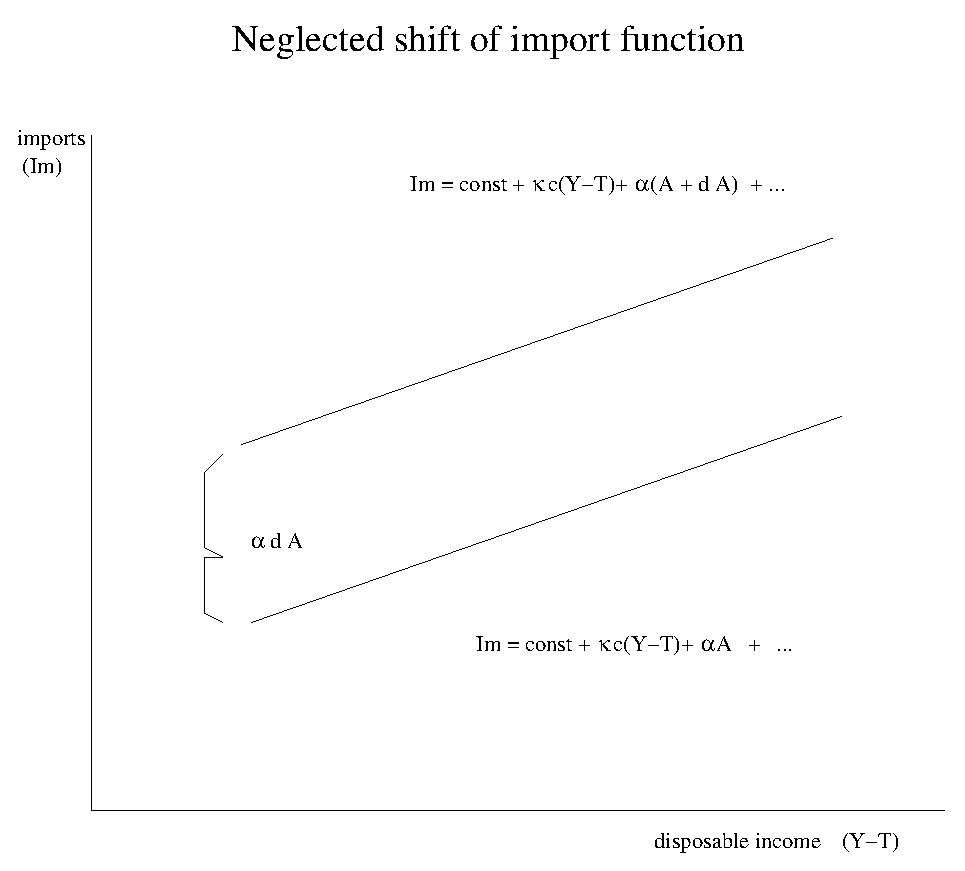
\includegraphics[scale=1.0]{import-1.eps}}
%\put(13,18){\mbox{Figure 1}}
%\end{picture}
% \put(20,0) \caption{}
%\end{figure}

\begin{figure}[h]
  \centering
  % Adjust the width fraction (e.g., 0.7 of text width) to size it perfectly
  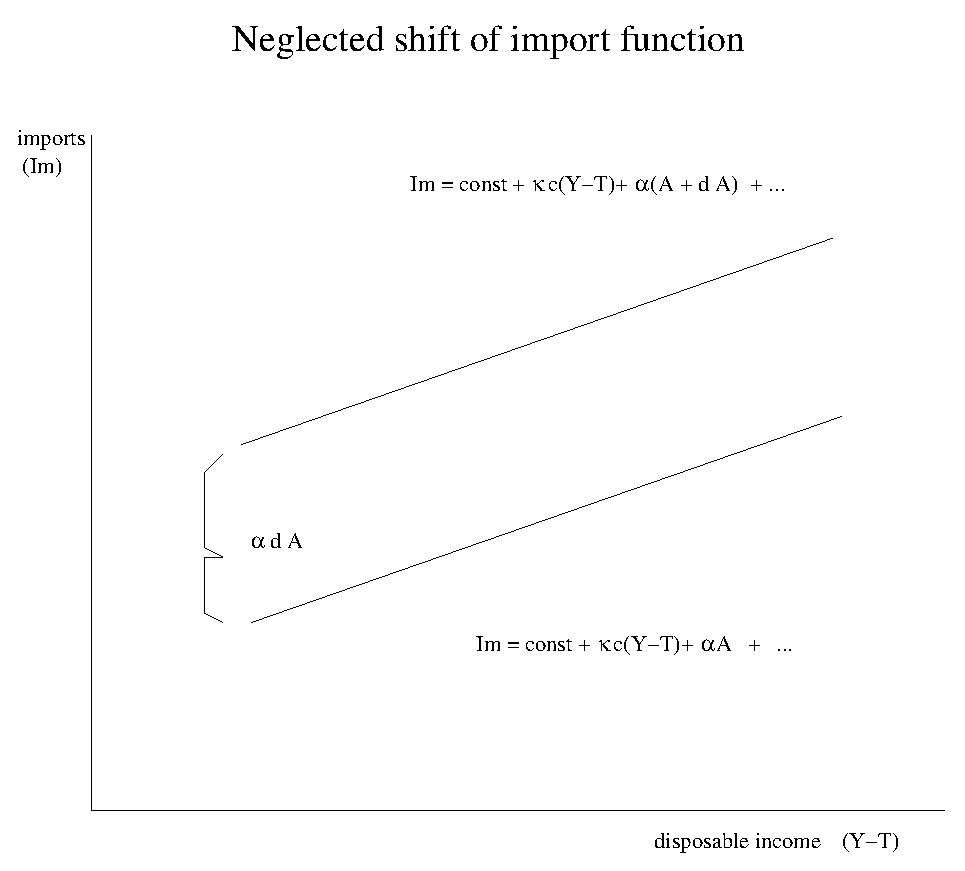
\includegraphics[width=0.7\textwidth]{import-1.eps}
%  \caption{Figure 1 Title or Description Go Here}
  \label{fig:import1}
\end{figure}

%\newpage
%\pagestyle{plain}


Neglecting shifts in the import function  is the flaw of current
macroeconomics I am discussing here. An import function that is free
of these defects would look like
\begin{eqnarray}
Im = const + \alpha A + \kappa C(Y-T) + \iota I + \epsilon Ex \label{eq:e4}\\
   = Im(\alpha A, \kappa C(Y-T), \iota I,\epsilon Ex)
\end{eqnarray}
with the marginal propensity m to import
\begin{eqnarray}
\noindent m & = & \frac{\partial Im}{\partial (Y-T)} \\
& = & \frac{\partial Im}{\partial
\kappa C(Y-T)}\frac{\partial \kappa C(Y-T)}{\partial (Y-T)} \\
& = & \frac{\partial Im}{\partial
\kappa C(Y-T)}\kappa\frac{ \partial C(Y-T)}{\partial (Y-T)} \\
& = & 1 \kappa c \\
& = & \kappa c.
\end{eqnarray}
for exogenous A, I and Ex subject to autonomous shifts, with
$\alpha$, $\iota$, $\kappa$,  $\epsilon$ restricted like x in $0
\leq x \leq 1$.

 Implicitly, I also have demonstrated here that imports should be
considered to depend on disposable income, Y-T, and not on current
income, Y.

\noindent For the marginal propensity to consume domestic
production, $c_d$, we obtain
\begin{equation}
c_d = (1-\kappa) c
\end{equation}

If we use the new import function (\ref{eq:e4}) to determine
\begin{equation}
dY
\end{equation}
then we shall obtain the correct multiplier for dA
\begin{equation}
\frac{1-\alpha}{1-c+m}
\end{equation}
instead of the false multiplier
\begin{equation}
\frac{1}{1-c+m}.
\end{equation}
Alternatively speaking, the traditional multiplier
\begin{equation}
\frac{1}{1-c+m}.
\end{equation}
should be applied to the modified impact or primary effect:
\begin{equation}
(1-\alpha)dA,
\end{equation}
and not be applied to $dA$ in order to obtain the correct value for
dY.

In the literature, one can find sophisticated steps undertaken in
order to improve the econometric specification of the import
function. But none in the direction of our present argument. A
particularly illustrative case is Brown (1970, pp. 232-235.).

\section{Debunking the Keynesian multiplier for open economies}

We shall now demonstrate the implications of the flaws of standard
macroeconomic analysis of open economies by proving two theorems. We
assume a fix-price world: In the underlying income model, commodity
prices, exchange rates and interest rates are held constant.


\subsection{Two theorems}

%\newtheorem{Keynes}{Theorem}
\begin{Keynes}
In open economies the Keynesian multiplier for public expenditures
may not only be smaller than 1 but may even be
negative.\footnote{The reader should note that we are arguing for a
fix-price world. Commodity prices, exchange rates and interest rates
are held constant. The ``smaller than 1'' part of theorem 1  could
be derived without our changes to the import function in a
flex-price setting with the Haavelmo condition dA=dT.}
\end{Keynes}

\noindent {\bf Proof:}
 \vspace{5mm}

 \noindent {\bf The Haavelmo-case}


\noindent Additional public expenditures have to be financed either
by current taxes, public debt or by additional money. Restrictions of
the European Monetary Union exclude financing by additional central
bank money. Financing by public debt implies financing by future
taxation. These financing restrictions are appropriately expressed
by the equation
\begin{equation} dA = dT.
\end{equation}
where the tax variable T comprises both current and future taxation
in present value terms.

We need to consider the total differential of the first equation:
\begin{equation}
dY = c(dY-dT) + dA - \alpha dA - m (dY-dT).
\end{equation}
%Here, $m = \kappa c$.
It may be combined with the Haavelmo restriction, $dA=dT$, and
solved for $dY$:
\begin{equation}
dY = (1 - \frac{\alpha}{1-c+m})dA \label{eq:e5}
\end{equation}

\noindent Depending on whether the import content parameter $\alpha$
is $=0$, $>0$, $=s+m$, or $>s+m$, the multiplier $1 -
\frac{\alpha}{s+m}$ in (\ref{eq:e5})  is
   $=1$, $<1$, $=0$, or $<0$.

 If the import content parameter $\alpha$ is zero, then we obtain
the classic Haavelmo-result of a multiplier of 1, thus replicating
the result of a prior note of mine. However, the multiplier for dA
becomes zero if
\begin{equation}
\alpha = 1-c + m.
\end{equation}
This condition restricts the value of the import content of public
expenditures, $\alpha$, to the sum of the marginal propensity to
save out of disposable income plus the marginal propensity to import
out of disposable income. The import content parameter $\alpha$ has
not to be equal to 1 in order to obtain a zero public expenditure
multiplier. If $\alpha > 1-c+m$ then the multiplier even becomes
negative. Thus, it is quite possible that public expenditure
expansion has a contractionary effect on the home economy.

\vspace{5mm}
 \noindent {\bf The case without the tax financing
constraint}

\noindent If the tax financing constraint is neglected, then dT=0
and
\begin{equation}
dY = \frac{1-\alpha}{1-c+m}dA.
\end{equation}


\noindent Since $\alpha \leq 1$, the multiplier cannot be negative
in the present case. With $m = \kappa c$, it is easy to show that
the multiplier $\frac{1-\alpha}{s+m}$ is smaller than 1 if and only
if $c \leq \frac{\alpha}{(1-\kappa)}$. For a multiplier smaller than
1 it is sufficient that $\alpha$ is larger than c. However, this is
not necessary. Even if $\alpha$ is merely a fraction of c, the
multiplier can still be smaller than 1. The multiplier even
converges to zero as the import content parameter of additional
public expenditures approaches 1.

%\newtheorem{Keynes2}{Theorem 2}
\begin{Keynes}
In open economies the Keynesian multiplier for autonomous
consumption, autonomous investment and exports will always be
non-negative but may be smaller than 1.\footnote{The reader should
note that this result does not involve a tax financing constraint.}
\end{Keynes}

\noindent {\bf Proof:}
 The demonstration and results for the preceding case of public expenditures without tax
financing apply not only to public expenditures, but also to
autonomous consumption, autonomous investment and autonomous
exports. Nothing forbids the replacement of the pair A and $\alpha$
by the pairs $C_a$ and $\kappa$, $I$ and $\iota$, $Ex$ and
$\epsilon$ respectively.


\subsection{Results} By taking into account the import content of
shifts in final demand, the prospects of Keynesian demand management
policies have become gloomier. The import content parameter can make
for unpleasant surprises in cases where the parameter is neglected,
unknown or where it cannot be known with certainty in advance. The
possibility of negative multipliers implies that national Keynesian
stabilisation policy can be counterproductive for the home country
and that the future of Keynesian demand management lies in
cooperative international schemes of stabilisation policies.


\section{Conclusion}

I have discussed a serious deficiency in the current practice of
formulating and analysing open economy macroeconomic models. The
problem may be seen as  one of misspecifying the import function in
open economy macroeconomics. However, to present the issue in this
way is likely to de-emphasise the relevance of the problem for
macroeconomic analysis. It is better to present the problem as a
case of an error in the specification of primary macroeconomic
effects in the analysis of demand management policies, although the
two visions are logically equivalent.

Needless to say that every open economy macroeconomic textbook needs
to be revised and that all open economy macroeconomic analyses that
have been presented in the past are flawed. The flaw consists in
neglecting the import content of autonomous shifts in the components
of final macroeconomic demand.

The specification error committed is not negligible because it is
enlarged by the very multiplier principle. If the specification
error is eliminated then the conventional multiplier results may
stop to hold not only quantitatively but even qualitatively. A
positive multiplier may turn into a negative one. Demand management
policies may become counterproductive for the home country. Thus the
potential consequences may be even more dramatic than those of the
Haavelmo-Theorem once were. The empirical likelihood for such
results has increased dramatically by way of internationalisation
and globalisation of economies in recent years. The future of
Keynesian demand management lies in cooperative stabilisation
schemes by which the contractive effects of import leakages are
overcome.

\bibliographystyle{plain}
\begin{thebibliography}{99}
T. Merritt Brown, Specification and Uses of Econometric Models,
Macmillan, 1970 \\
Colin Clark, The National Income of Australia, London 1939 \\
 Trygve Haavelmo, Multiplier effects of a Balanced
Budget, Econometrica,
Vol. 13, 1945, pp. 31ff. \\
Richard F. Kahn, The relation of home investment to unemployment,
Economic Journal, June 1931, pp. 173-198. \\
John Maynard Keynes, General Theory of
Employment, Interest and Money, London 1936 \\
Nikolaus K.A. L�ufer, Haavelmo's theorem in open economies: the
insulation effect, unpublished manuscript, May 2009 \\
Nikolaus K.A. L�ufer, Undermining the case for Keynesian Demand
Management: Is the public expenditure multiplier negative?
unpublished manuscript, August 2009 \\
James E. Meade, Theory of International Economic Policy, Vol. I, The
Balance of Payments, 1951, repr. 1963, with Mathematical Supplement
1951, repr. 1960. \\
Fritz Machlup, International Trade and the
National Income Multiplier, Blakiston Co., Philadelphia 1943, \\
 Fritz Machlup, Period Analysis and Multiplier Theory, Quarterly
 Journal of Economics, Vol. 54, Nov. 1939, pp. 1-27. \\
 Erich Schneider, Einf�hrung in die Wirtschaftstheorie, III. Teil,
 Geld, Kredit, Volkseinkommen und Besch�ftigung, 4. verbesserte u.
 erweiterte Auflage 1957. \\
%German Federal Statistical Office, Press release No. 302 from
%August, 17th, 2009.
\end{thebibliography}
\end{document}
